\subsection{Linux kernel sources}

\begin{frame}
  \frametitle{Location of kernel sources}
  \begin{itemize}
  \item The official versions of the Linux kernel, as released by Linus
    Torvalds, are available at \url{http://www.kernel.org}
    \begin{itemize}
    \item These versions follow the development model of the kernel
    \item However, they may not contain the latest development from a
      specific area yet. Some features in development might not be
      ready for mainline inclusion yet.
    \end{itemize}
  \item Many chip vendors supply their own kernel sources
    \begin{itemize}
    \item Focusing on hardware support first
    \item Can have a very important delta with mainline Linux
    \item Useful only when mainline hasn't caught up yet.
    \end{itemize}
  \item Many kernel sub-communities maintain their own kernel, with
    usually newer but less stable features
    \begin{itemize}
    \item Architecture communities (ARM, MIPS, PowerPC, etc.), device
      drivers communities (I2C, SPI, USB, PCI, network, etc.), other
      communities (real-time, etc.)
    \item No official releases, only development trees are available.
    \end{itemize}
  \end{itemize}
\end{frame}

\begin{frame}
  \frametitle{Getting Linux sources}
  \begin{itemize}
  \item The kernel sources are available from
    \url{http://kernel.org/pub/linux/kernel} as {\bf full tarballs}
    (complete kernel sources) and {\bf patches} (differences between
    two kernel versions).
  \item However, more and more people use the \code{git} version
    control system. Absolutely needed for kernel development!
    \begin{itemize}
    \item Fetch the entire kernel sources and history\\
      \code{git clone git://git.kernel.org/pub/scm/linux/kernel/git/torvalds/linux.git}
    \item Create a branch that starts at a specific stable version\\
      \code{git checkout -b <name-of-branch> v3.11}
    \item Web interface available at
      \url{http://git.kernel.org/cgit/linux/kernel/git/torvalds/linux.git/tree/}.
    \item Read more about Git at \url{http://git-scm.com/}
    \end{itemize}
  \end{itemize}
\end{frame}

\begin{frame}
  \frametitle{Working with git: SSD storage needed for serious work}
  \begin{columns}
  \column{0.6\textwidth}
  For all work with \code{git}, but especially on big projects such as
  the Linux kernel...
  \begin{itemize}
  \item Having a fast disk will dramatically speed up most \code{git}
    operations.
  \item Ask your boss to order an SSD disk for your laptop. It will make
    you more productive.
  \item If you are in a Bootlin public session, you already have an
    SSD disk!
  \end{itemize}
  \column{0.4\textwidth}
  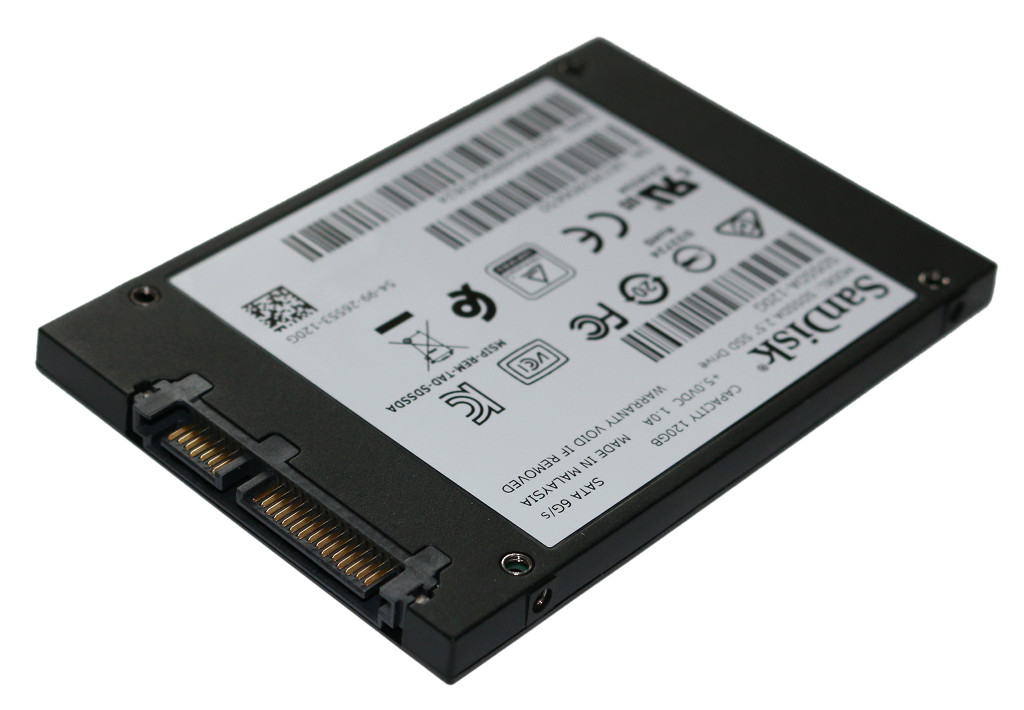
\includegraphics[width=\textwidth]{slides/sysdev-linux-intro-sources/sandisk-ssd-back.jpg}
  % Source: https://commons.wikimedia.org/wiki/File:Sandisk_SSD_and_connectors.jpg
  % Created by Bootlin
  \end{columns}
\end{frame}


\begin{frame}
  \frametitle{Linux kernel size (1)}
  \begin{itemize}
  \item Linux 4.11 sources:\\
    \begin{itemize}
	\item 57994 files (\code{git ls-files | wc -l})
	\item 23144003 lines (\code{wc -l $(git ls-files)})
	\item 675576310 bytes (\code{wc -c $(git ls-files)})
    \end{itemize}
  \item Minimum Linux 4.11 compiled kernel size,
        booting to a shell on the ARM Versatile board:
    	405,464 bytes (compressed), 1,112,264 bytes (raw)
  \item Why are these sources so big?\\
    Because they include thousands of device drivers, many network
    protocols, support many architectures and filesystems...
  \item The Linux core (scheduler, memory management...) is pretty
    small!
  \end{itemize}
\end{frame}

\begin{frame}
  \frametitle{Linux kernel size (2)}
  As of kernel version 4.6 (in lines).
  \begin{columns}
    \column{0.5\textwidth}
    \begin{itemize}
    \item \kdir{drivers}: 57.0\%
    \item \kdir{arch}: 16.3\%
    \item \kdir{fs}: 5.5\%
    \item \kdir{sound}: 4.4\%
    \item \kdir{net}: 4.3\%
    \item \kdir{include}: 3.5\%
    \item \kdir{Documentation}: 2.8\%
    \item \kdir{tools}: 1.3\%
    \item \kdir{kernel}: 1.2\%
    \end{itemize}
    \column{0.5\textwidth}
    \begin{itemize}
    \item \kdir{firmware}: 0.6\%
    \item \kdir{lib}: 0.5\%
    \item \kdir{mm}: 0.5\%
    \item \kdir{scripts}: 0.4\%
    \item \kdir{crypto}: 0.4\%
    \item \kdir{security}: 0.3\%
    \item \kdir{block}: 0.1\%
    \item ...
    \end{itemize}
  \end{columns}
\end{frame}
